In diesem Kapitel werden die aufgenommenen Messungen ausgewertet und deren Bedeutung graphisch analysiert. Wie in Kapitel \ref{software} erwähnt, werden zweidimensionale Ausgaben, wie die x- und y-Ausgabe des Gyroskops, in einem Scatterhistogramm dargestellt, welches es ermöglicht, die Dichteverteilung einzusehen. 



%Notizen:
%
%Die folgenden Graphen unterscheiden sich in ihrer Darstellung: Zum einen wurden Gyroskop, Beschleunigungssensors, Winkel und Center of Mass in sog. Scatterhistogrammen geplottet, siehe Abb \ref{Gyr},\ref{Acc},\ref{Angle}. Der Hauptplot ist ein scatter-Plot, welcher die Verteilung auf der X verglichen zur Y-Achse zeigt. An den Rändern sind jeweils die Histogramme der Achsen aufgetragen, welche die Wahrscheinlichkeitsverteilung angeben. Dabei ist die Annahme, dass ein stabilierer Gang eine steilere Wahrscheinlichkeitsverteilung hervorbringt, da sich die Aufnahmepunkte in der Mitte häufen müssten. Eine flache Verteilungskurve würde im Gegenzug bedeuten, dass NAO während dem Gang große Schwankungen aufweist und deshalb instabiler läuft.
%
%Es lässt sich eine Tendenz erkennen, dass der Gang mit Magneten stabiler ist, als ohne. Außerdem zeichnet sich das 20\,\% MAP durch besonders gute Stabilität hab. 
%
%Der Strom wurde in Histogrammen aufgetragen, welche die relative Häufigkeit des Stroms während der Messung aufzeigt. Die Graphen \ref{AnklePitch_Current_links},\ref{AnklePitch_Current_rechts},\ref{AnkleRoll_Current_links},\ref{AnkleRoll_Current_rechts} sind unterteilt in zwei Arten von Plots. Einerseits ist ein Histogramm mit jeweils 20 Säulen zu sehen. Diese wurde mit der Wahrscheinlichkeitsdichtefunktion von Matlab (pdf) ergänzt, um die Verteilung besser einsehen zu können.
%
%Die Annahme ist, dass ein höherer Strom mehr Reibungs- oder Haftwiderstand bedeuten. Leider ist die Datenlage hier sehr uneindeutig. 

\begin{figure}[tb]
	\centering
	\begin{adjustwidth}{-0.2\linewidth}{-0.2\linewidth}
	\begin{subfigure}[c]{.5\linewidth}
		\centering
		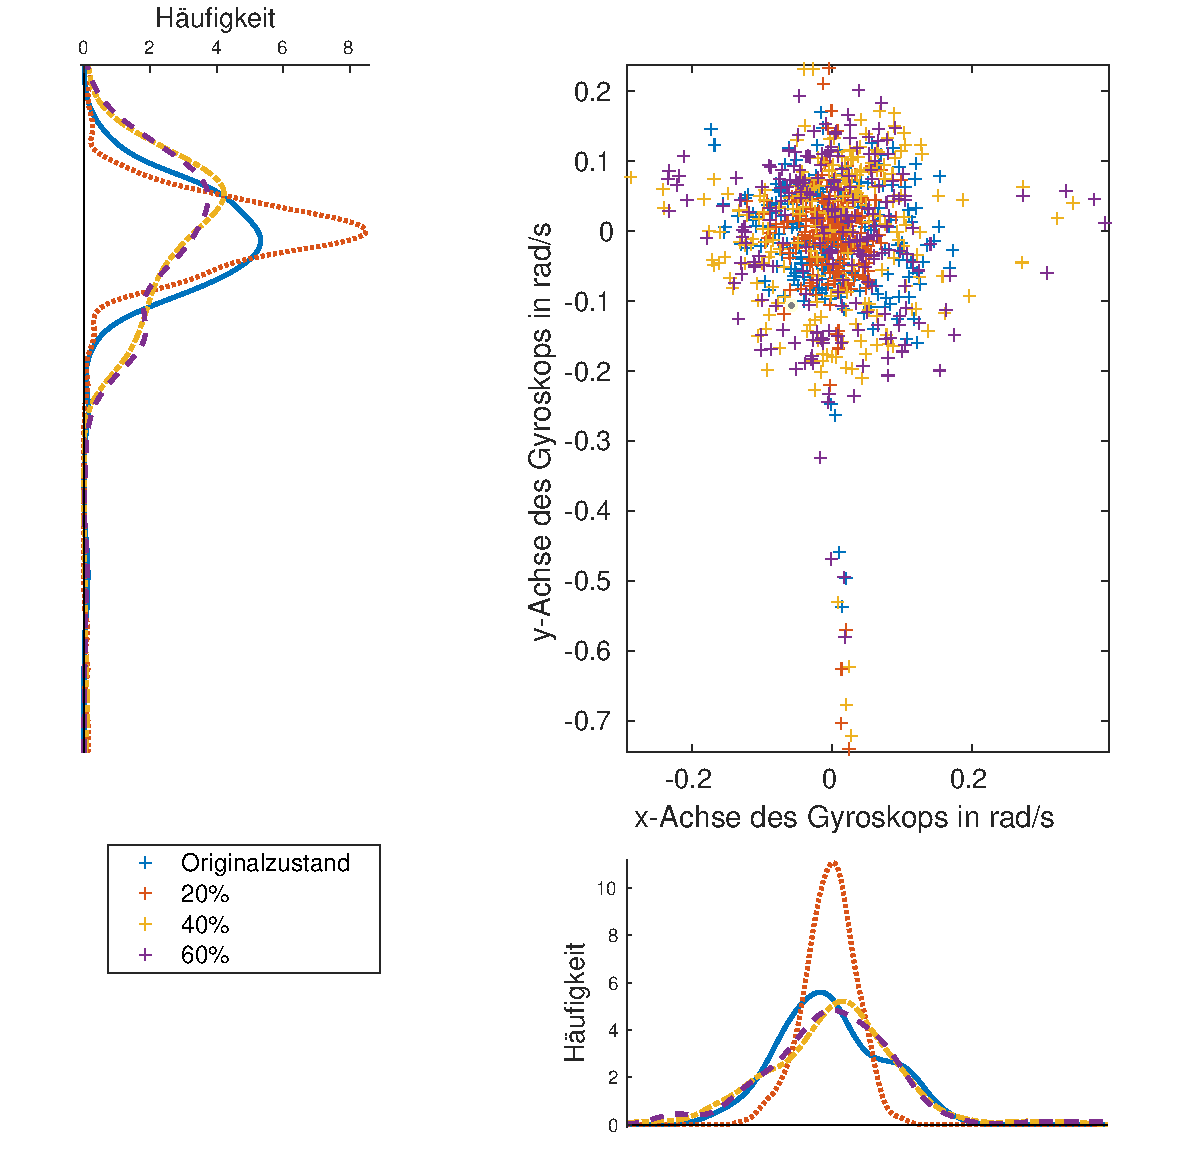
\includegraphics[width=\linewidth]{Bilder/Gyr_Grund_20_40_60_ohneM.pdf}
		\vspace{5pt}
	\end{subfigure}
	\hfill
	\begin{subfigure}[c]{.5\linewidth}
		\centering
		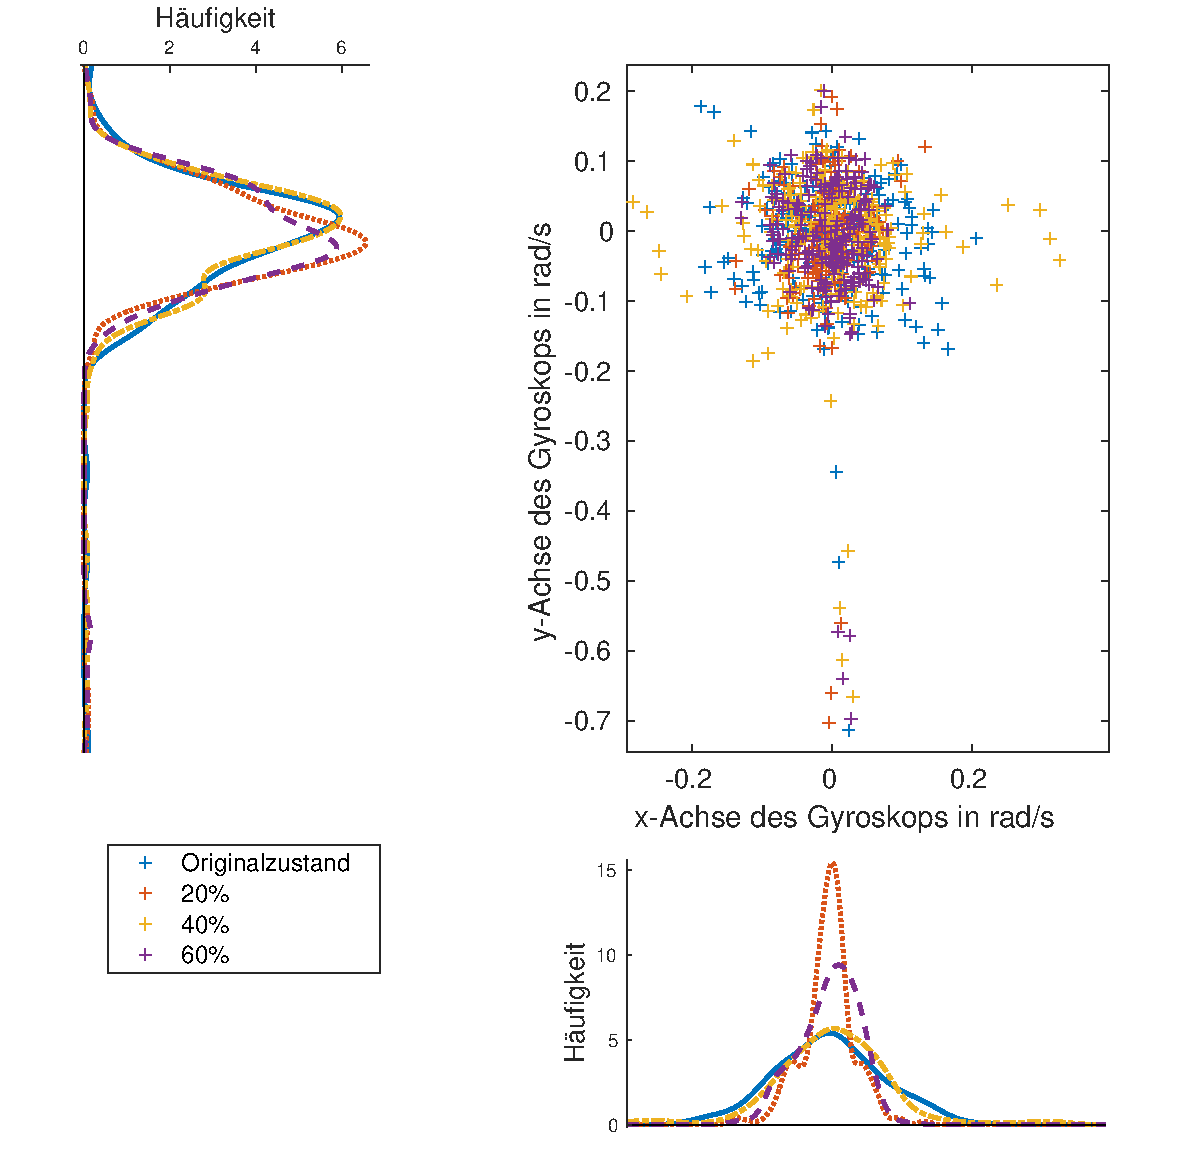
\includegraphics[width=\linewidth]{Bilder/Gyr_Grund_20_40_60_mitM.pdf}
		\vspace{5pt}
	\end{subfigure}
	\end{adjustwidth}
	\caption{Ausgabe des Gyroskops, x-Achse auf y-Achse, links ohne Magneten, rechts mit Magneten}\label{Gyr}
\end{figure}
\begin{figure}[htb]
	\centering
	\begin{adjustwidth}{-0.2\linewidth}{-0.2\linewidth}
	\hspace{5pt}
	\begin{subfigure}[c]{.45\linewidth}
		\centering
		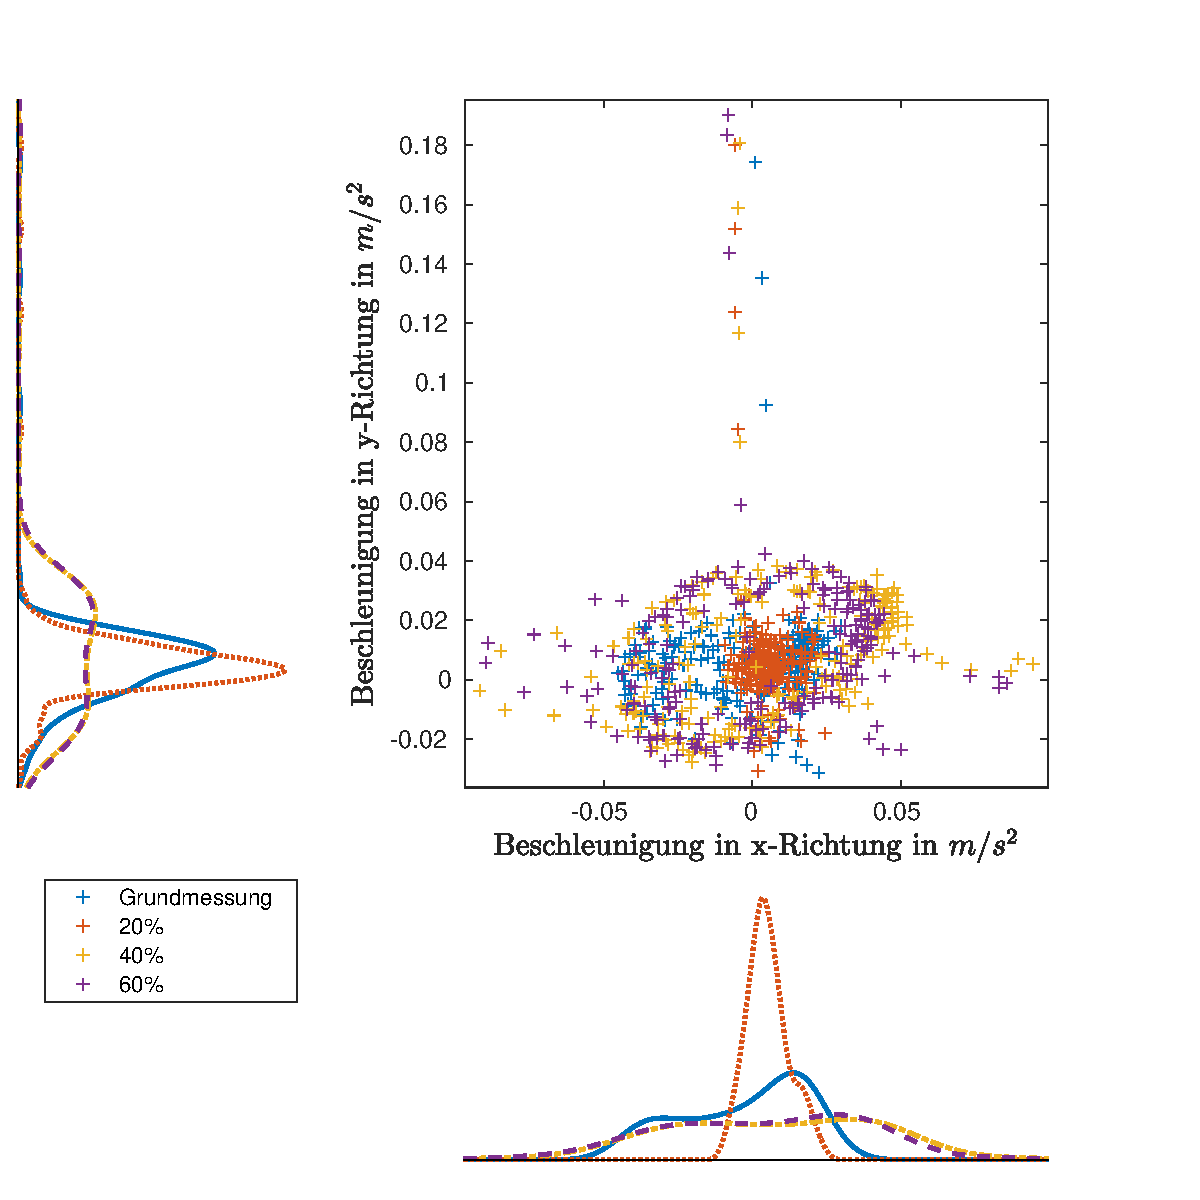
\includegraphics[width=\linewidth]{Bilder/Beschleunigung_Grund_20_40_60_ohneM.pdf}
		\vspace{5pt}
	\end{subfigure}
	%\hfill
	\hspace{20pt}
	\begin{subfigure}[c]{.45\linewidth}
		\centering
		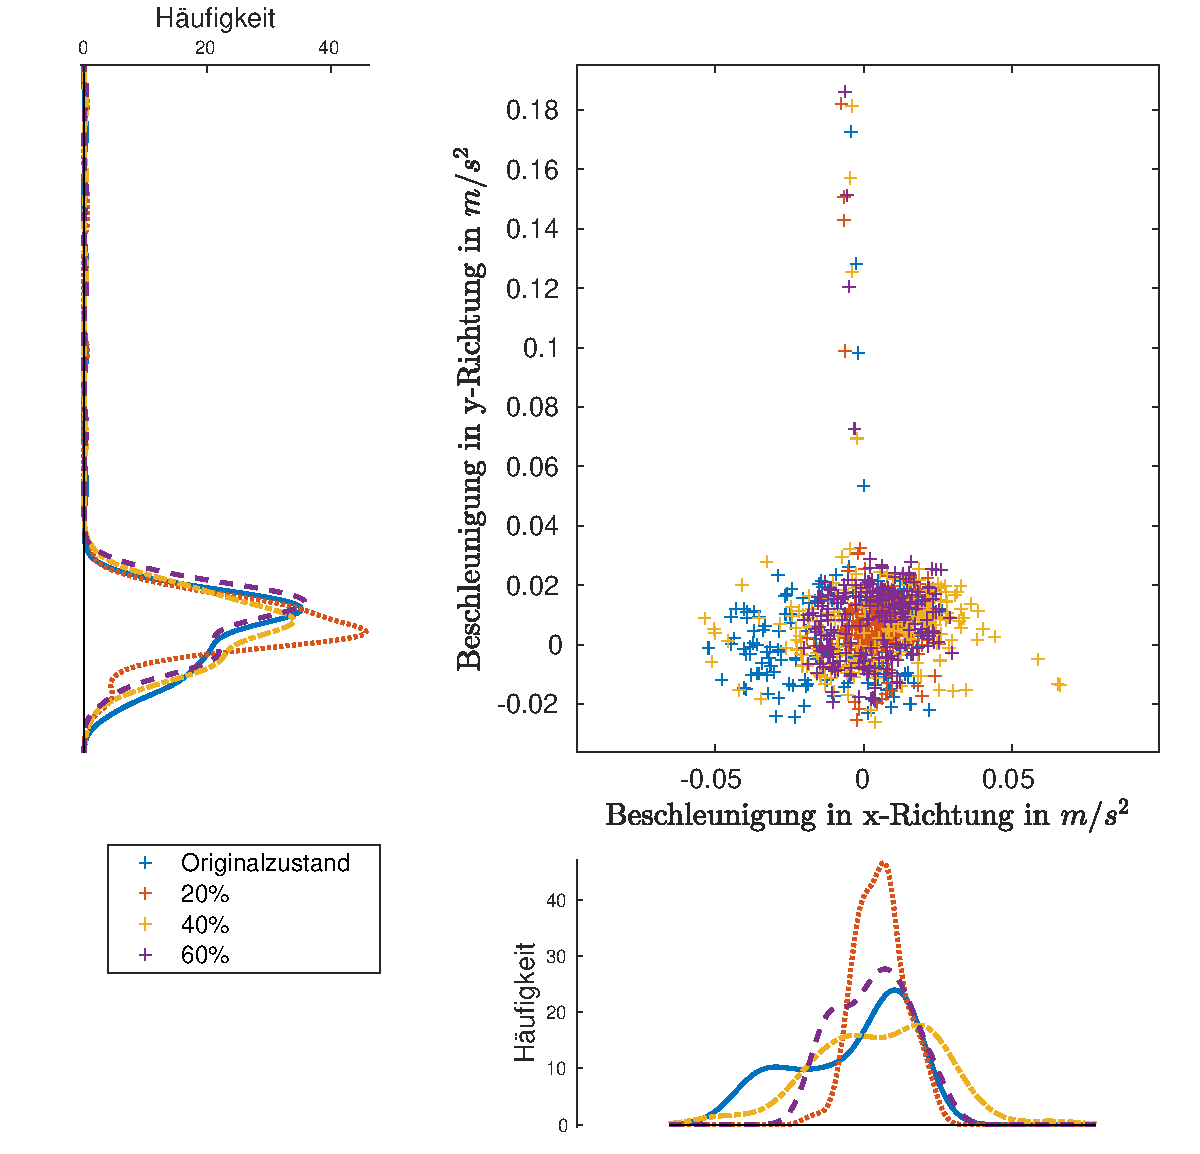
\includegraphics[width=\linewidth]{Bilder/Beschleunigung_Grund_20_40_60_mitM.pdf}
		\vspace{5pt}
	\end{subfigure}
	\end{adjustwidth}
	\caption{Ausgabe des Beschleunigungssensors, x-Achse auf y-Achse aufgetragen, links ohne Magneten, rechts mit Magneten} \label{Acc}
\end{figure}
\begin{figure}[htb]
	\centering
	\begin{adjustwidth}{-0.2\linewidth}{-0.2\linewidth}
		\hspace{5pt}
		\begin{subfigure}[c]{.45\linewidth}
			\centering
			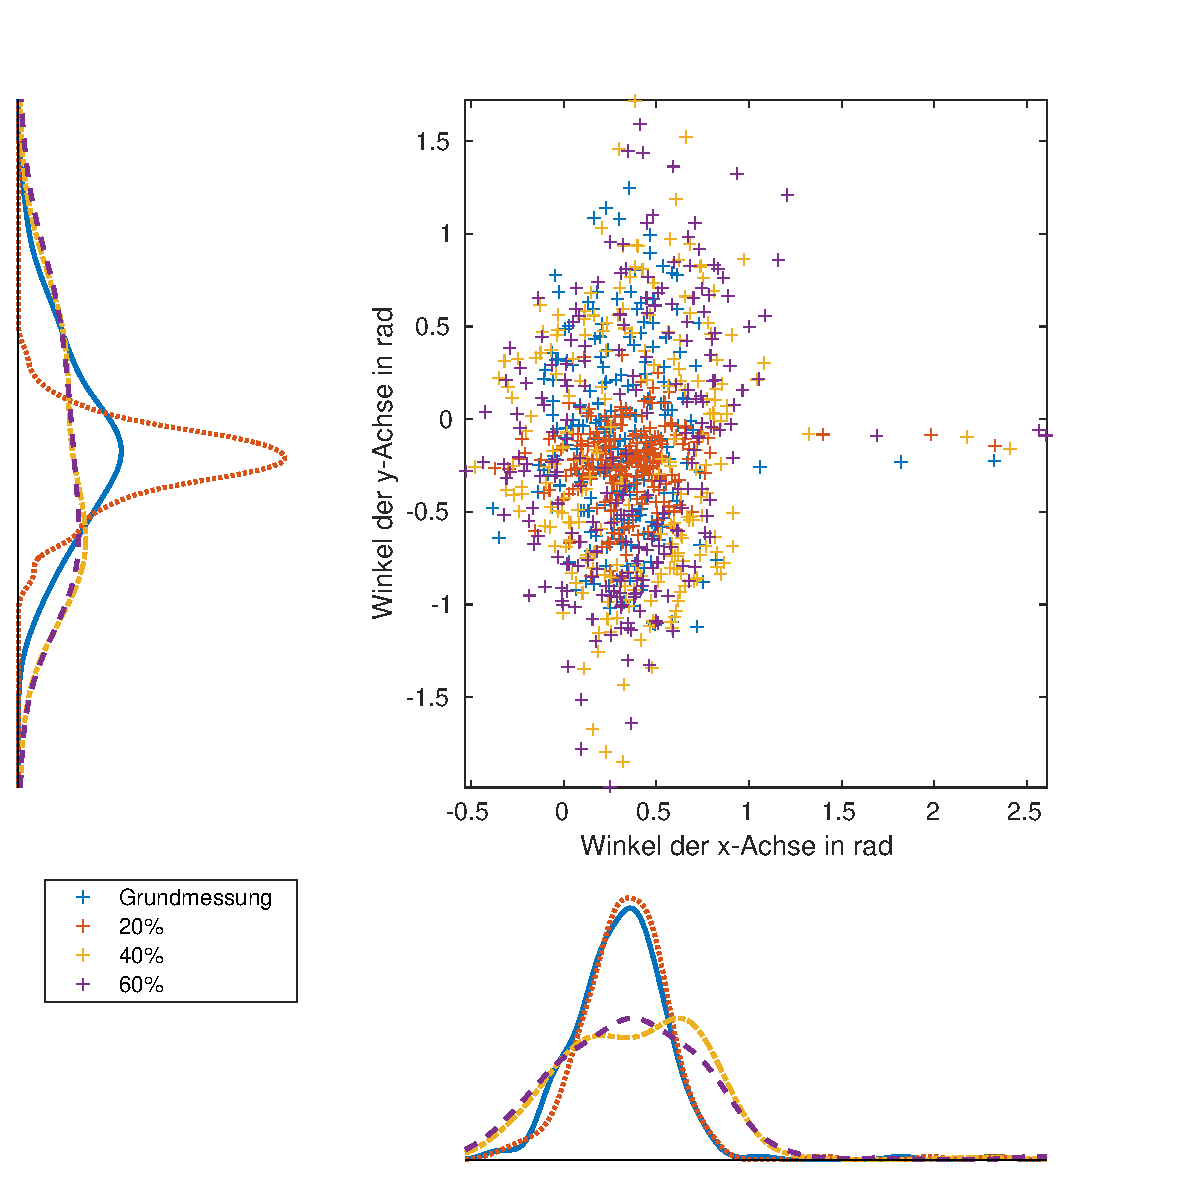
\includegraphics[width=\linewidth]{Bilder/Winkel_Grund_20_40_60_ohneM.pdf}
			\vspace{5pt}
		\end{subfigure}
		\hspace{20pt}
		%\hfill
		\begin{subfigure}[c]{.45\linewidth}
			\centering
			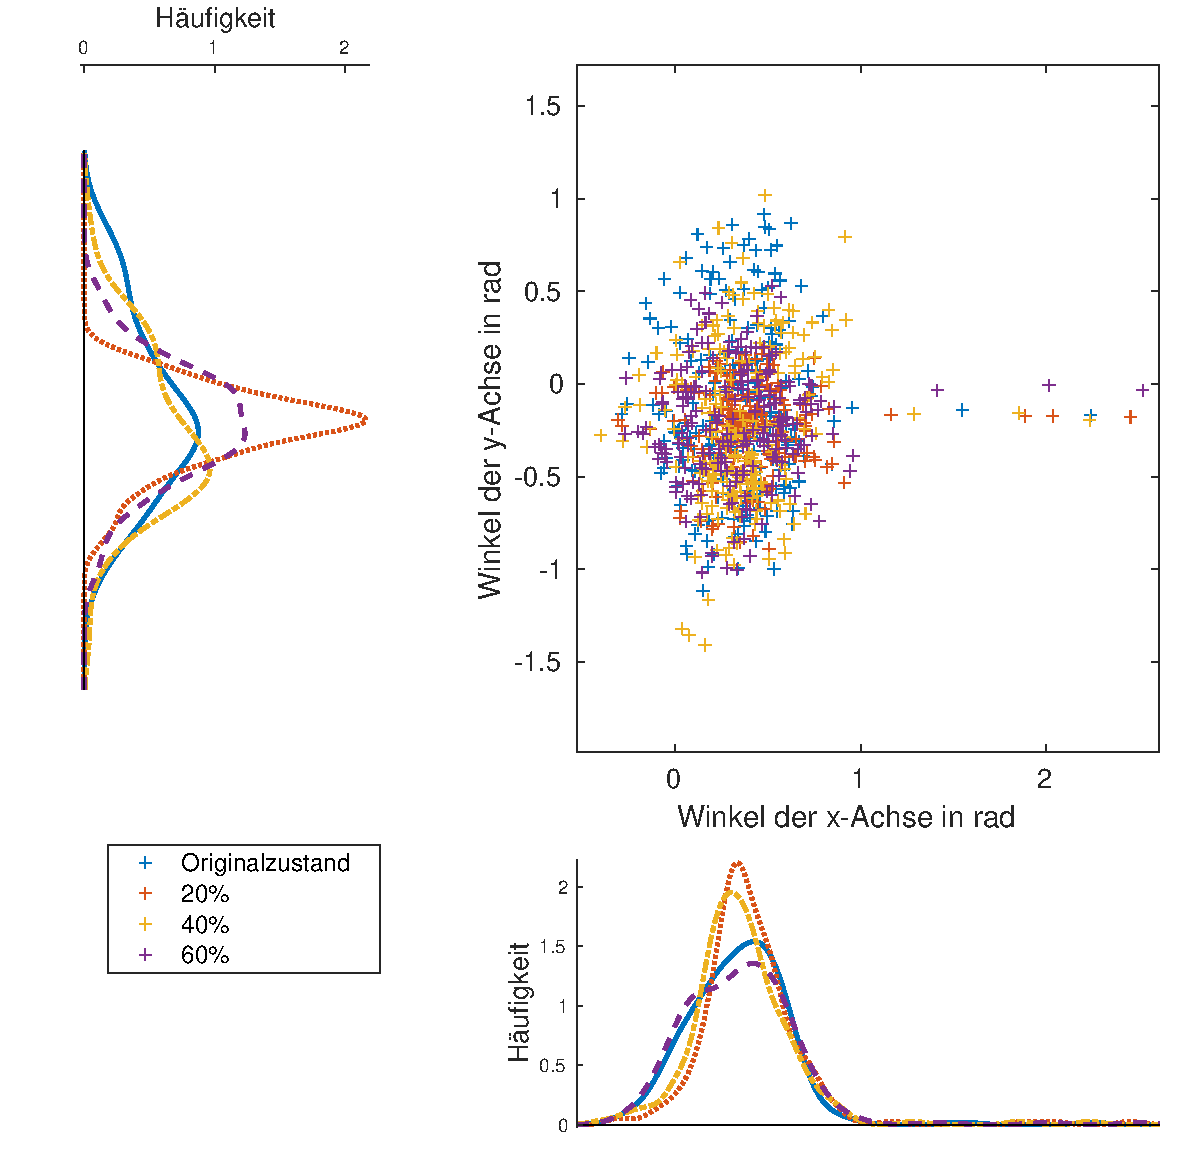
\includegraphics[width=\linewidth]{Bilder/Winkel_Grund_20_40_60_mitM.pdf}
			\vspace{5pt}
		\end{subfigure}
	\end{adjustwidth}
	\caption{Echtzeit errechneter Winkel, x-Achse auf y-Achse aufgetragen, links ohne Magneten, rechts mit Magneten} \label{Angle}
\end{figure}

\begin{figure}[tb]
	\centering
	\begin{adjustwidth}{-0.2\linewidth}{-0.2\linewidth}
		\hspace{5pt}
		\begin{subfigure}[c]{.45\linewidth}
			\centering
			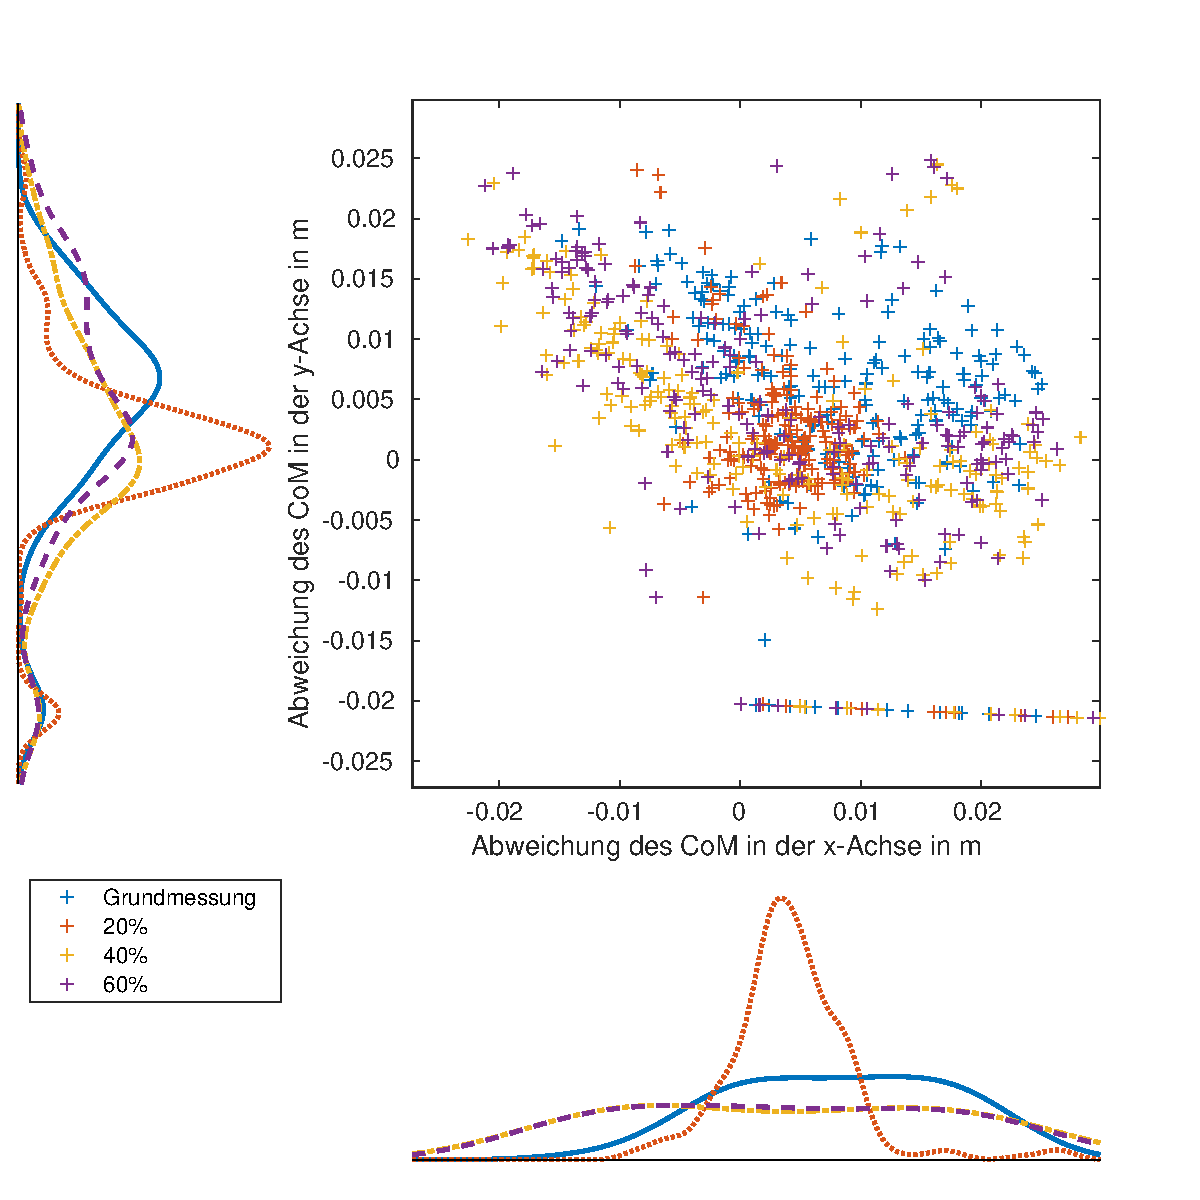
\includegraphics[width=\linewidth]{Bilder/links_CoM_ohneM.pdf}
			\vspace{5pt}
		\end{subfigure}
		\hspace{20pt}
		%\hfill
		\begin{subfigure}[c]{.45\linewidth}
			\centering
			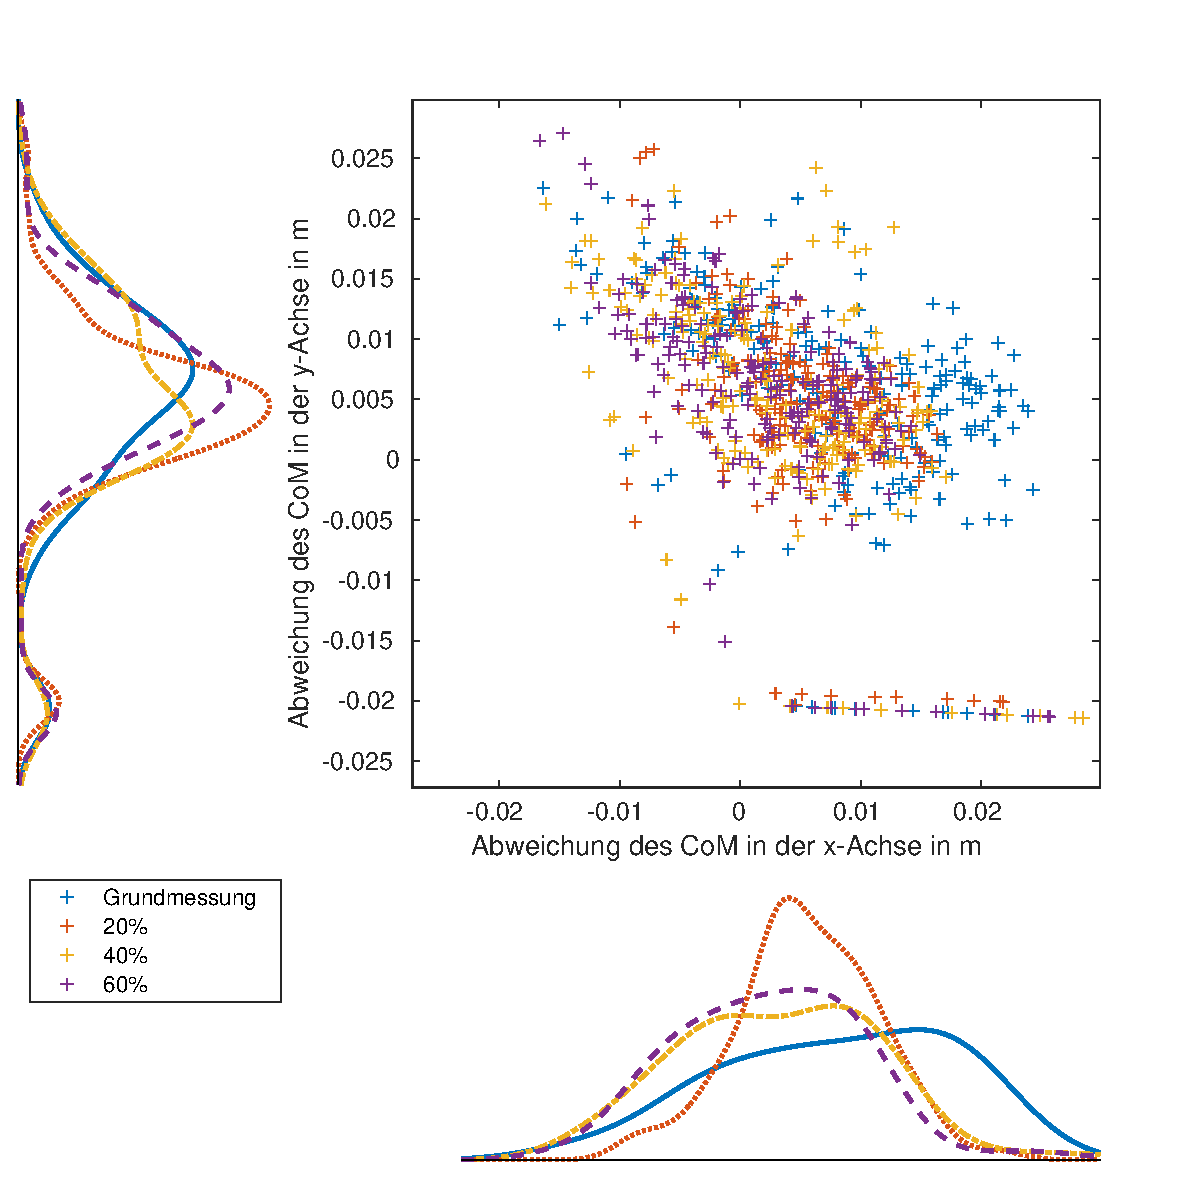
\includegraphics[width=\linewidth]{Bilder/links_CoM_mitM.pdf}
			\vspace{5pt}
		\end{subfigure}
	\end{adjustwidth}
	\caption{Linker errechneter Massenschwerpunkt aufgenommen durch die FSR, x-Achse auf y-Achse aufgetragen, links ohne Magneten, rechts mit Magneten} \label{CoM_links}
\end{figure}
\begin{figure}[tb]
	\centering
	\begin{adjustwidth}{-0.2\linewidth}{-0.2\linewidth}
		\hspace{5pt}
		\begin{subfigure}[c]{.45\linewidth}
			\centering
			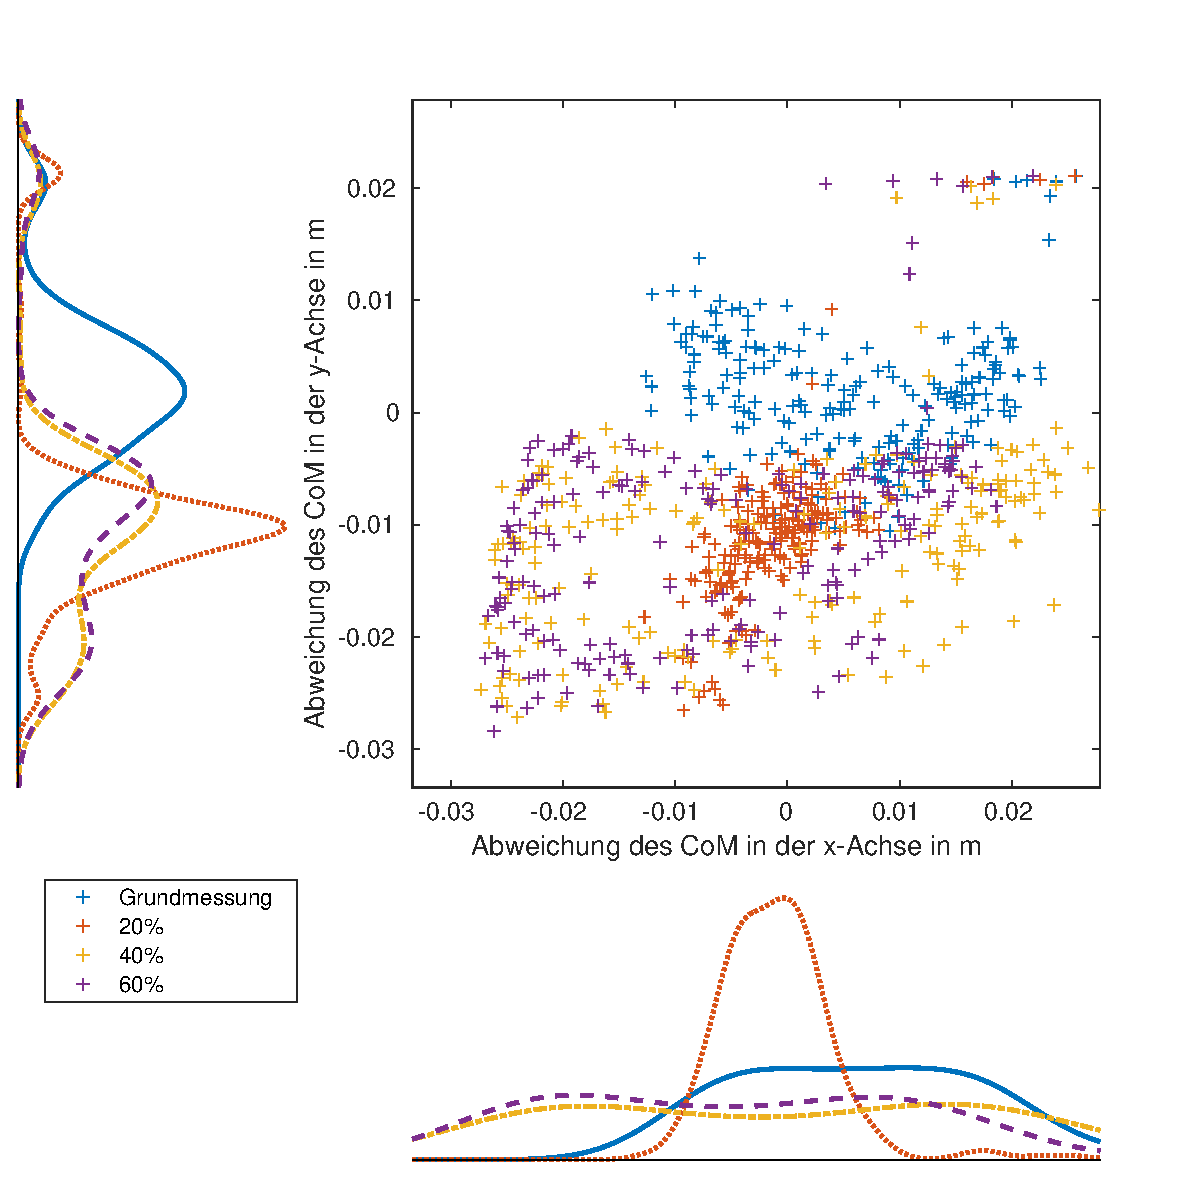
\includegraphics[width=\linewidth]{Bilder/rechts_CoM_ohneM.pdf}
			\vspace{5pt}
		\end{subfigure}
		\hspace{20pt}
		%\hfill
		\begin{subfigure}[c]{.45\linewidth}
			\centering
			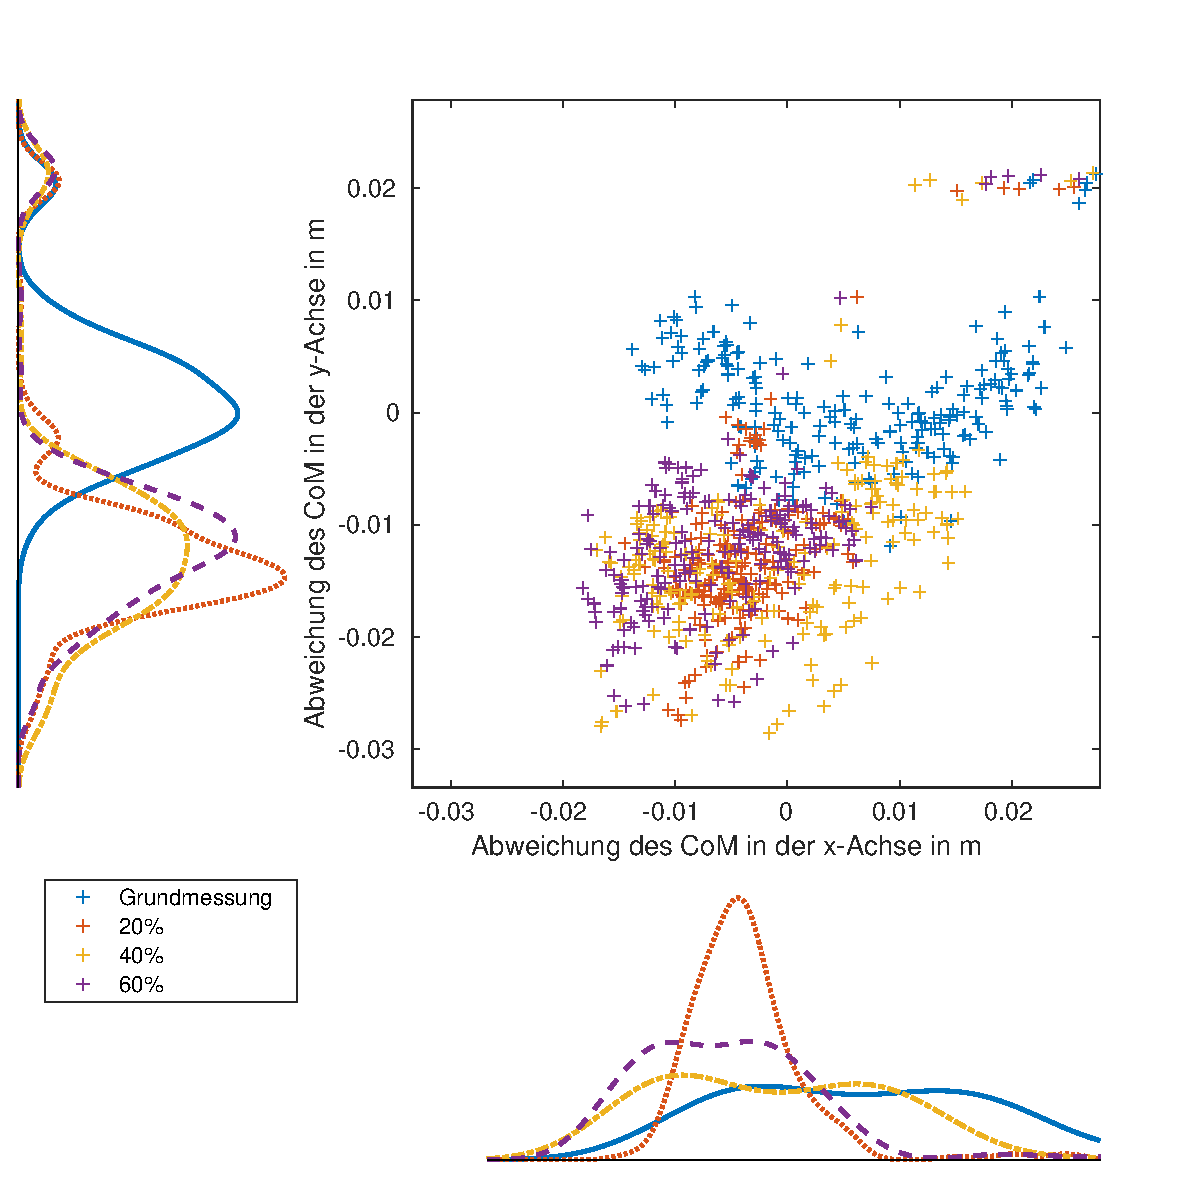
\includegraphics[width=\linewidth]{Bilder/rechts_CoM_mitM.pdf}
			\vspace{5pt}
		\end{subfigure}
	\end{adjustwidth}
	\caption{Rechter errechneter Massenschwerpunkt aufgenommen durch die FSR, x-Achse auf y-Achse aufgetragen, links ohne Magneten, rechts mit Magneten} \label{CoM_rechts}
\end{figure}

\begin{figure}[tb]
	\centering
%	\begin{adjustwidth}{-0.2\linewidth}{-0.2\linewidth}
%		\hspace{5pt}
		\begin{subfigure}[c]{.9\linewidth}
			\centering
			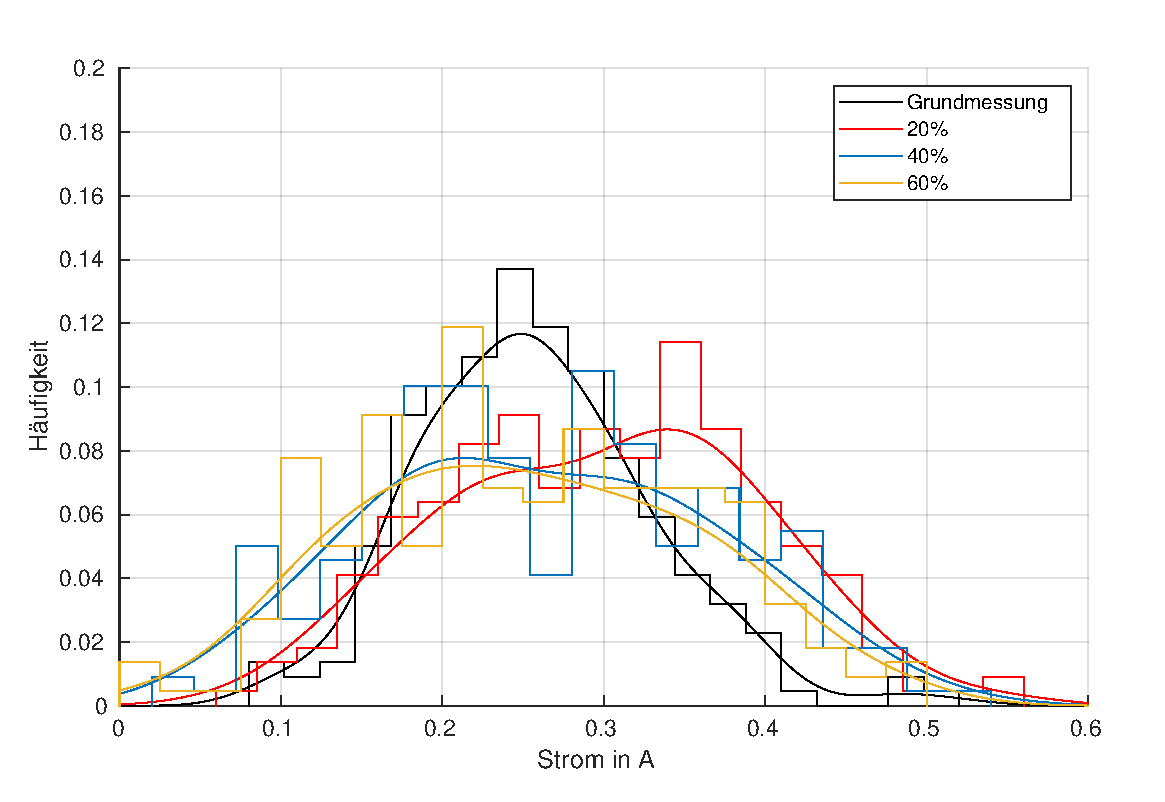
\includegraphics[width=\linewidth]{Bilder/links_Current_AnklePitch_ohneM.pdf}
%			\vspace{5pt}
		\end{subfigure}
%		\hspace{20pt}
%		\hfill
		\begin{subfigure}[c]{.9\linewidth}
			\centering
			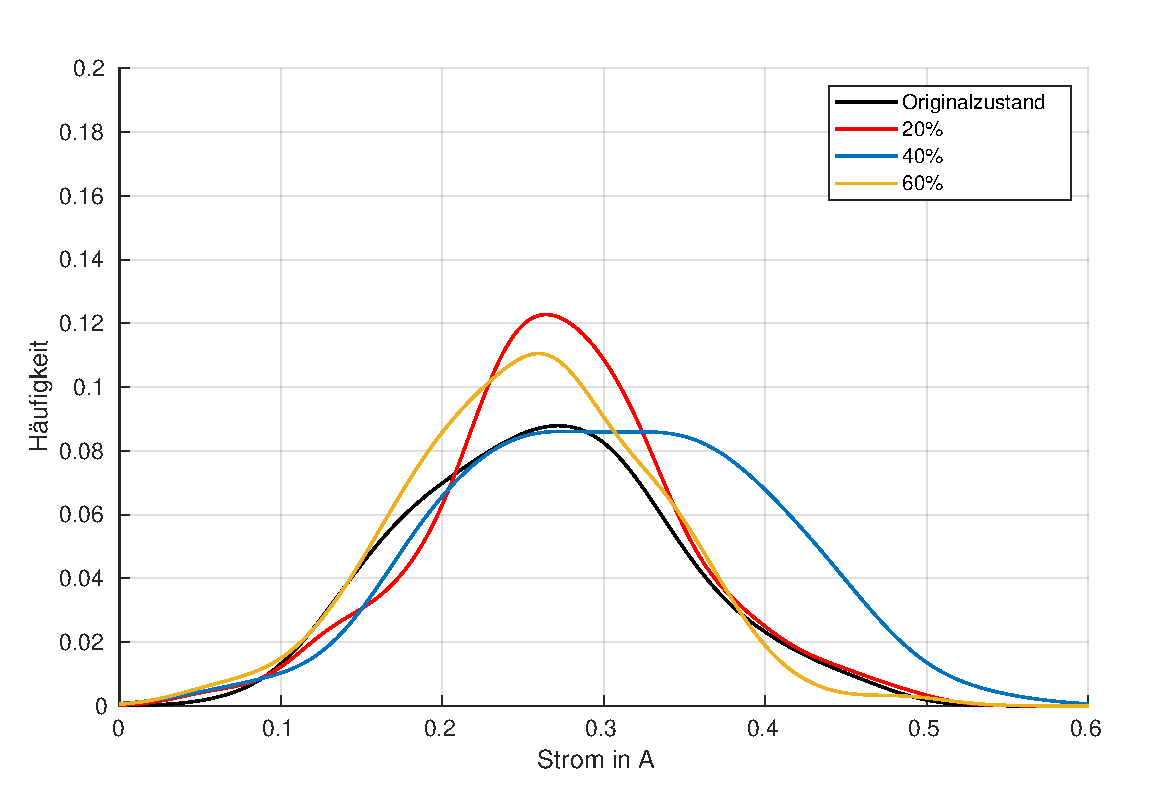
\includegraphics[width=\linewidth]{Bilder/links_Current_AnklePitch_mitM.pdf}
%			\vspace{5pt}
		\end{subfigure}
%	\end{adjustwidth}
	\caption{AnklePitch gemessener Strom im linken Fuß, Strom in Ampère aufgetragen auf die Häufigkeit. Das Histogramm wurde ergänzt durch eine Wahrscheinlichkeitsdichtefunktion. Der obere Graph sind die Aufnahmen ohne Magneten, der untere mit Magneten.} \label{AnklePitch_Current_links}
\end{figure}
\begin{figure}[tb]
	\centering
%	\begin{adjustwidth}{-0.2\linewidth}{-0.2\linewidth}
%		\hspace{5pt}
		\begin{subfigure}[c]{.9\linewidth}
			\centering
			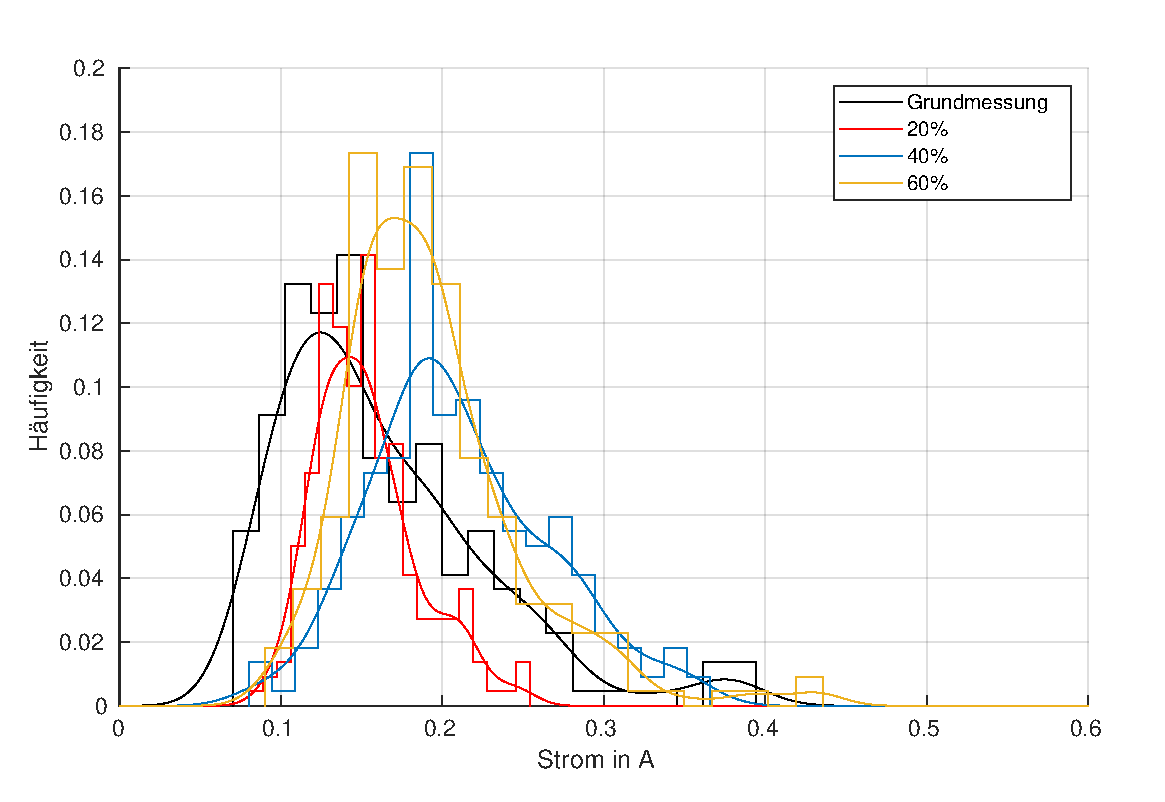
\includegraphics[width=\linewidth]{Bilder/rechts_Current_AnklePitch_ohneM.pdf}
			\vspace{5pt}
		\end{subfigure}
%		\hspace{20pt}
		\hfill
		\begin{subfigure}[c]{.9\linewidth}
			\centering
			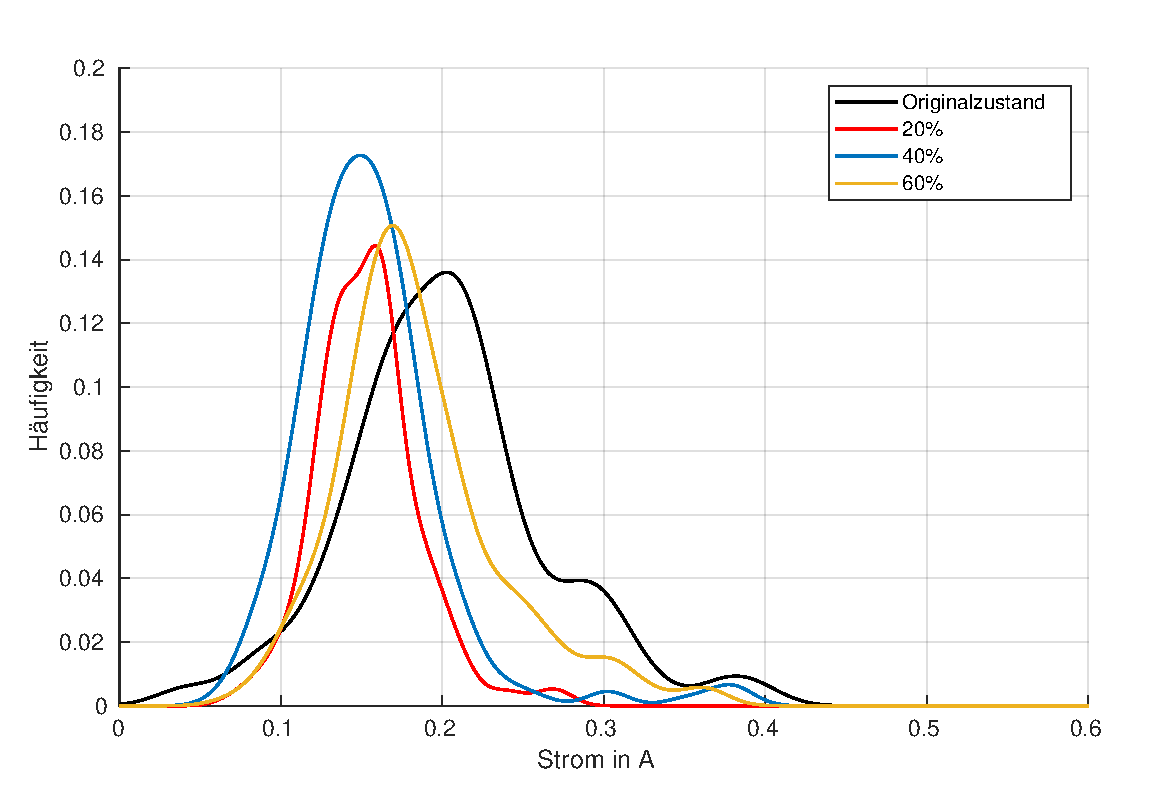
\includegraphics[width=\linewidth]{Bilder/rechts_Current_AnklePitch_mitM.pdf}
			\vspace{5pt}
		\end{subfigure}
%	\end{adjustwidth}
	\caption{AnklePitch gemessener Strom im rechter Fuß, Strom in Ampère aufgetragen auf die Häufigkeit. Das Histogramm wurde ergänzt durch eine Wahrscheinlichkeitsdichtefunktion. Der obere Graph sind die Aufnahmen ohne Magneten, der untere mit Magneten.} \label{AnklePitch_Current_rechts}
\end{figure}

\begin{figure}[tb]
	\centering
	%	\begin{adjustwidth}{-0.2\linewidth}{-0.2\linewidth}
	%		\hspace{5pt}
	\begin{subfigure}[c]{.9\linewidth}
		\centering
		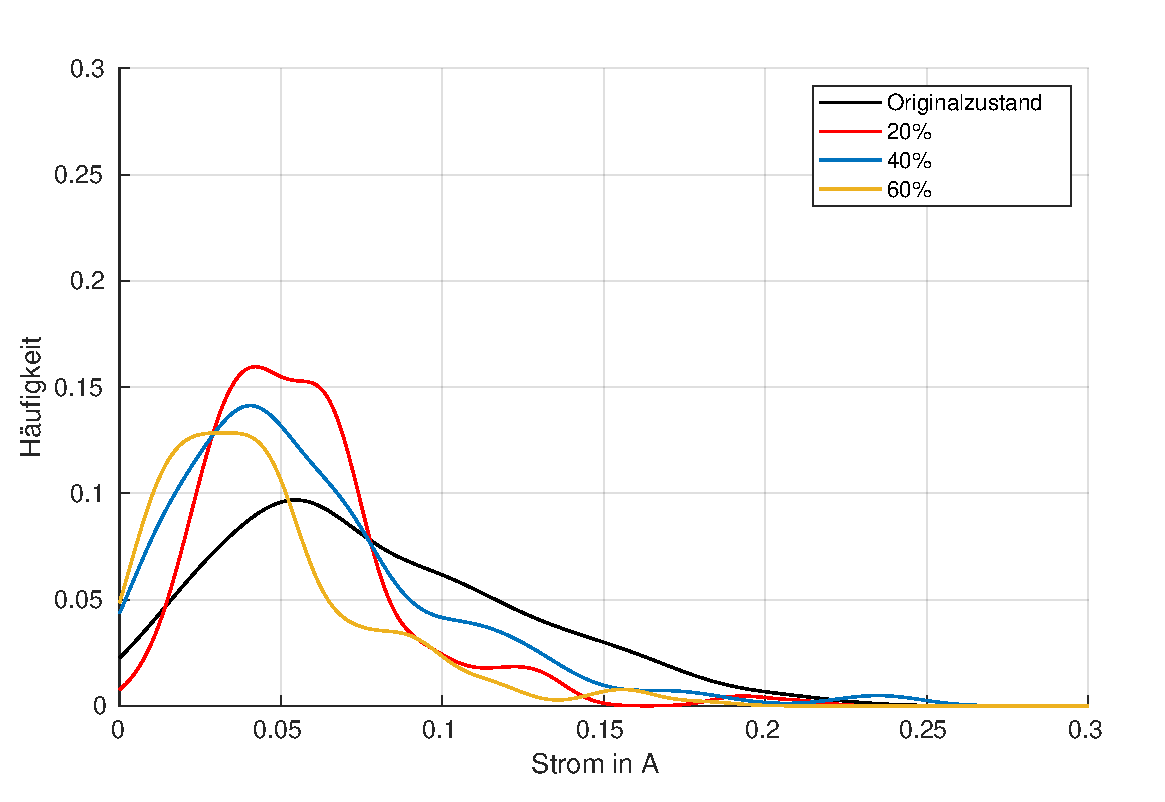
\includegraphics[width=\linewidth]{Bilder/links_Current_AnkleRoll_ohneM.pdf}
		%			\vspace{5pt}
	\end{subfigure}
	%		\hspace{20pt}
	%		\hfill
	\begin{subfigure}[c]{.9\linewidth}
		\centering
		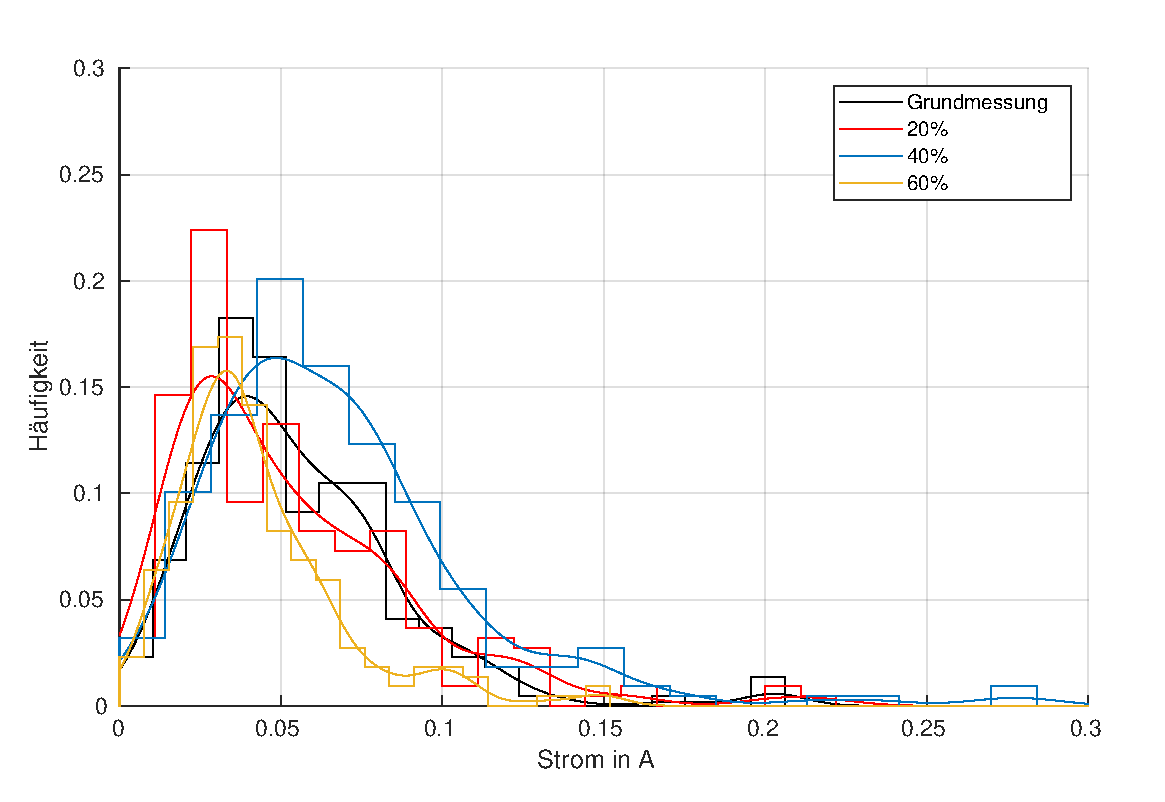
\includegraphics[width=\linewidth]{Bilder/links_Current_AnkleRoll_mitM.pdf}
		%			\vspace{5pt}
	\end{subfigure}
	%	\end{adjustwidth}
	\caption{AnkleRoll gemessener Strom im linken Fuß, Strom in Ampère aufgetragen auf die Häufigkeit. Das Histogramm wurde ergänzt durch eine Wahrscheinlichkeitsdichtefunktion. Der obere Graph sind die Aufnahmen ohne Magneten, der untere mit Magneten.} \label{AnkleRoll_Current_links}
\end{figure}
\begin{figure}[tb]
	\centering
	%	\begin{adjustwidth}{-0.2\linewidth}{-0.2\linewidth}
	%		\hspace{5pt}
	\begin{subfigure}[c]{.9\linewidth}
		\centering
		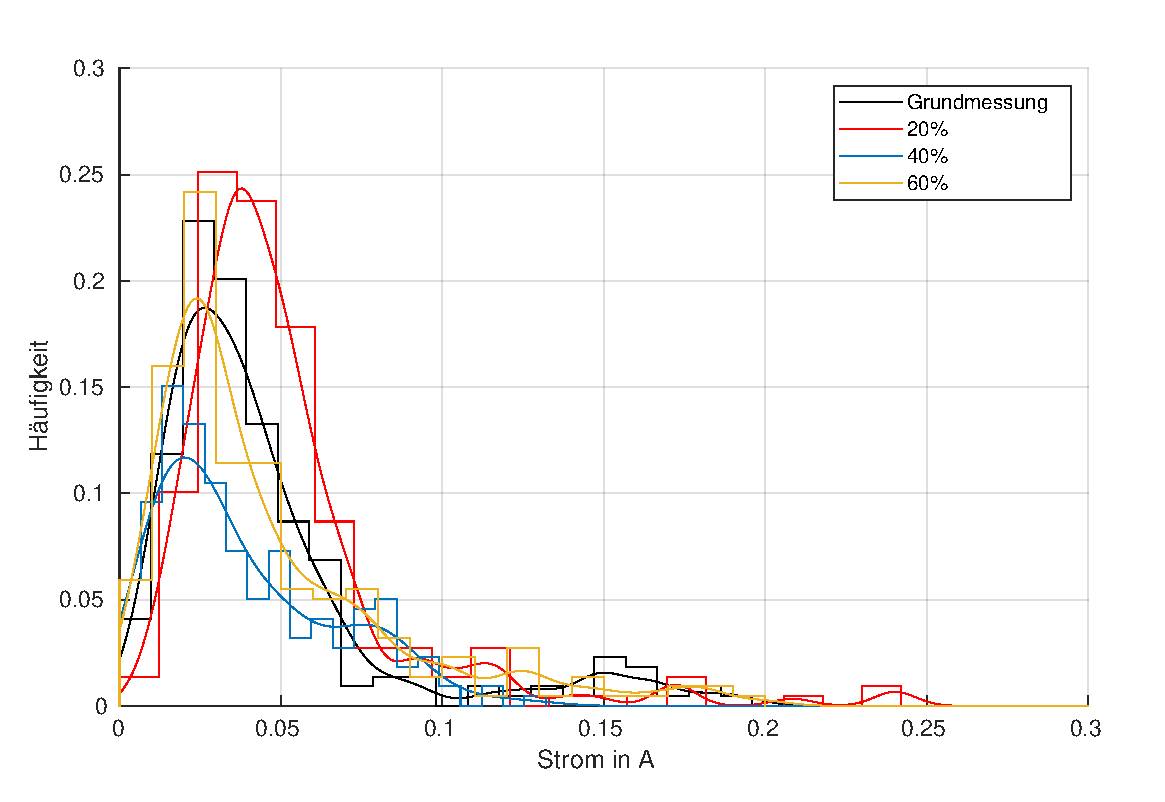
\includegraphics[width=\linewidth]{Bilder/rechts_Current_AnkleRoll_ohneM.pdf}
		\vspace{5pt}
	\end{subfigure}
	%		\hspace{20pt}
	\hfill
	\begin{subfigure}[c]{.9\linewidth}
		\centering
		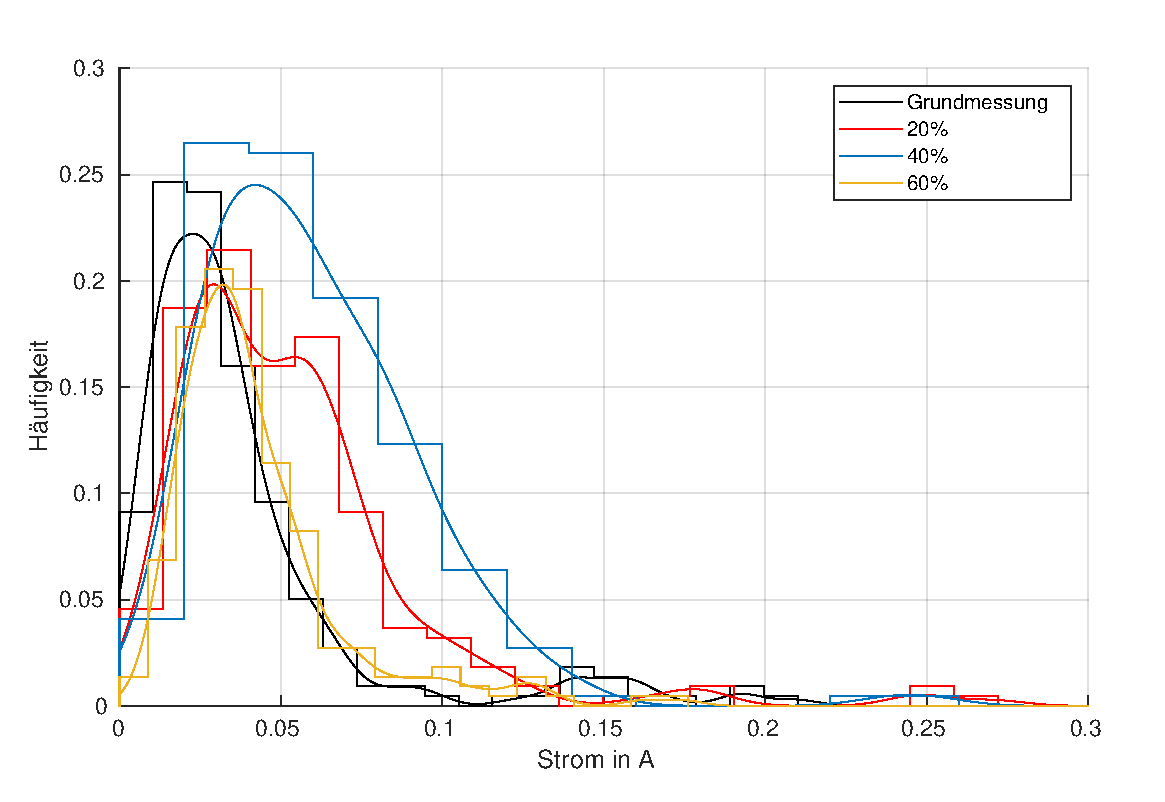
\includegraphics[width=\linewidth]{Bilder/rechts_Current_AnkleRoll_mitM.pdf}
		\vspace{5pt}
	\end{subfigure}
	%	\end{adjustwidth}
	\caption{AnkleRoll gemessener Strom im rechter Fuß, Strom in Ampère aufgetragen auf die Häufigkeit. Das Histogramm wurde ergänzt durch eine Wahrscheinlichkeitsdichtefunktion. Der obere Graph sind die Aufnahmen ohne Magneten, der untere mit Magneten.} \label{AnkleRoll_Current_rechts}
\end{figure}

%\subsection{Messungen von AnkleRoll zum Test}
%Die Messungen von LAnkleRoll und RAnkleRoll, zu sehen in Abb. \ref{hardware_llegjoint} und \ref{hardware_rlegjoint} wurden 20 mal wiederholt und mit den normalen Schuhen von Nao vollzogen. Dabei legte er in etwa eine Strecke von $0,8 \unit{m}$ auf der Rampe im flachen Zustand zurück. Insgesamt wurden alle verfügbaren Messwerte von AnkleRoll aufgezeichnet, das sind pro Aktor 6 Messwerte. Temperatur, Stiffness und Temperatur Status erwiesen sich als Konstant und daher nicht entscheidend, um einen Unterschied der Bodenbeschaffenheit oder Sohlen erkennen zu können. Stiffness ist immer auf $100\%$ während dem Gang. 
%Der Befehl für diesen Lauf war der moveTo() Befehl, welcher nicht weiter verändert wurde (kommt in den Theorieteil).
%
%
%In Abb. \ref{AnkleRoll_links_act} und \ref{AnkleRoll_rechts_act} sind die Messdaten von jeweils einem Fuß des Messwertes Position/Actuator abgebildet. Hier ist zu sehen, dass die Anfangswerte sich aufspalten, in positive und einmal in negative Winkelangaben. Dies ist der Tatsache geschuldet, dass die Funktion moveTo() per Zufall Nao mit dem linken oder mit dem rechten Fuß beginnen lässt. 
%
%Dies wurde für Abb. \ref{AnkleRoll_beide_act_sens_links_anfang} und \ref{AnkleRoll_beide_act_sens_rechts_anfang} sortiert. In ersterer Abbildung beginnt Nao mit dem linken Fuß. Da die Hüfte sich für den ersten Schritt nach rechts bewegen muss, verschiebt sich die Position beider Gelenke in die Negativrichtung, der Winkel wird absolut gemessen, wie in Abb \ref{hardware_llegjoint} und \ref{hardware_rlegjoint} zu sehen ist. 
%
%Außerdem sind in Abb. \ref{AnkleRoll_beide_act_sens_links_anfang} und \ref{AnkleRoll_beide_act_sens_rechts_anfang} neben den Messwerten von Position Actuator in schwarz auch die von Position Sensor in blau gezeigt. \textcolor{red}{Was diese beiden Messwerte genau unterscheidet und ob einer von moveTo() vorgegeben wird, ist noch zu entscheiden.} Der bedeutenste Unterschied ist zu Beginn der Aufnahmen. Die Position/Actuator Messung beginnt nahe 0, während Position/Sensor für den jeweiligen Fuß bei einem Wert über Null oder unter Null anfängt. 
%
%Es ist eindeutig zu erkennen, dass die Messungen erst nach der Sortierung des Anfangsschrittes ein regelmäßiges Bild ergeben. 
%
%Der Strom, welcher die Gelenke einsetzen müssen um das gewollte Ergebnis zu erzielen, scheint eine mögliche, vergleichbare Aufnahmegröße für unterschiedliche Sohlen und Umgebungen des Nao zu sein. In Abb. \ref{AnkleRoll_beide_current_links_anfang} und \ref{AnkleRoll_beide_act_sens_rechts_anfang} ist der Messwert Current aufgeteilt in Anfangsschritte gezeigt. Hier ist der Unterschied, mit welchem Fuß der erste Schritt gemacht wird, nicht so gravierend, wie bei den vorherigen Messwerten. Allerdings zeichnet sich eine Tendenz ab, dass der linke Fuß, hier in schwarz, einen höheren Strom beansprucht, als der rechte Fuß. Dies könnte dem beobachteten Fehlgang des Naos und dem zusätzlichen Geräusch bei jedem zweiten Schritt geschultet sein. Bei normaler Einstellung und ohne Korrektur würde dieser Nao einen Bogen nach rechts laufen. Um dies auszugleichen wurden bei moveTo() Anpassungen hinzugefügt.   
%
%\begin{figure}[tb]
%	\centering
%	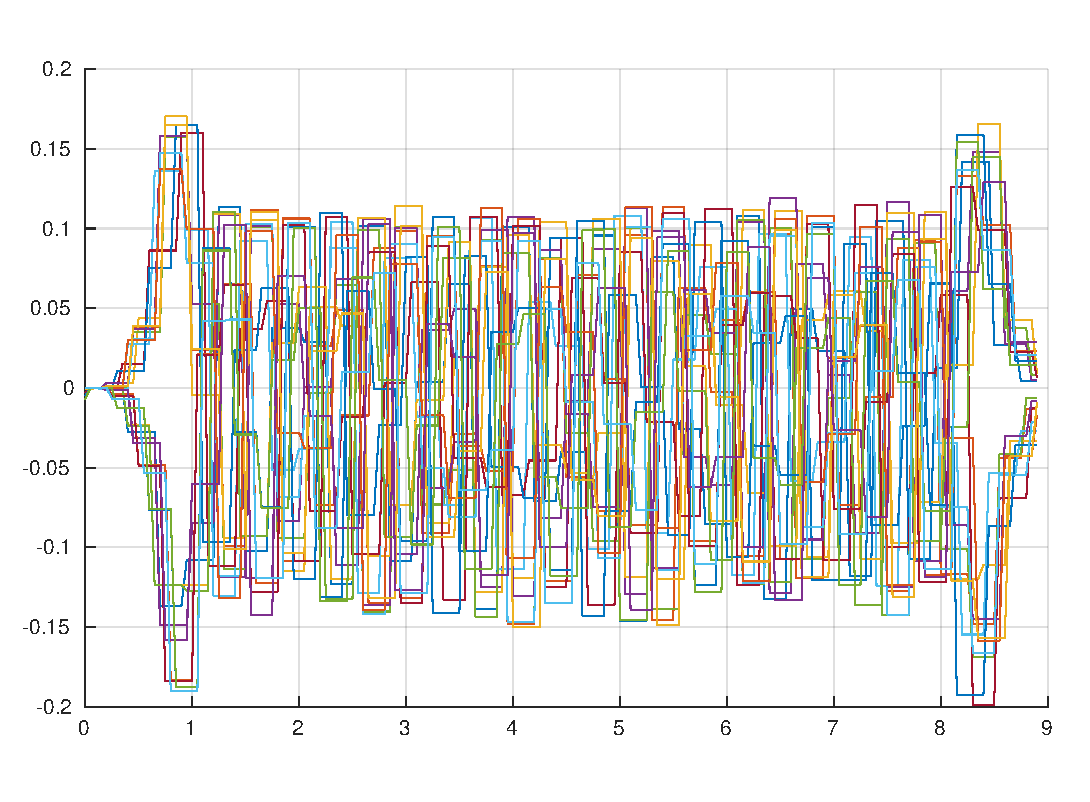
\includegraphics[width=1\linewidth]{Bilder/AnkleRoll_links_act.pdf}
%	\caption{AnkleRoll Messwert Position Actuator des linken Fußes}
%	\label{AnkleRoll_links_act}
%\end{figure}
%
%\begin{figure}[tb]
%	\centering
%	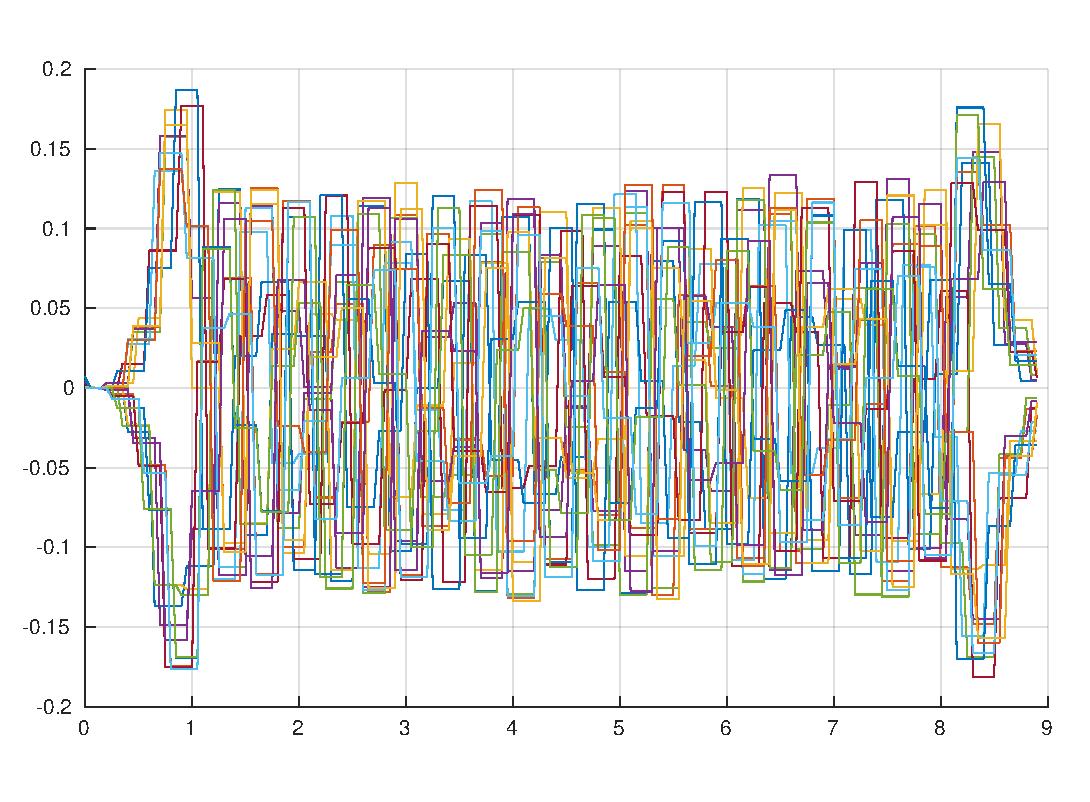
\includegraphics[width=1\linewidth]{Bilder/AnkleRoll_rechts_act.pdf}
%	\caption{AnkleRoll Messwert Position Actuator des rechten Fußes}
%	\label{AnkleRoll_rechts_act}
%\end{figure}
%\begin{figure}[tb]
%	\centering
%	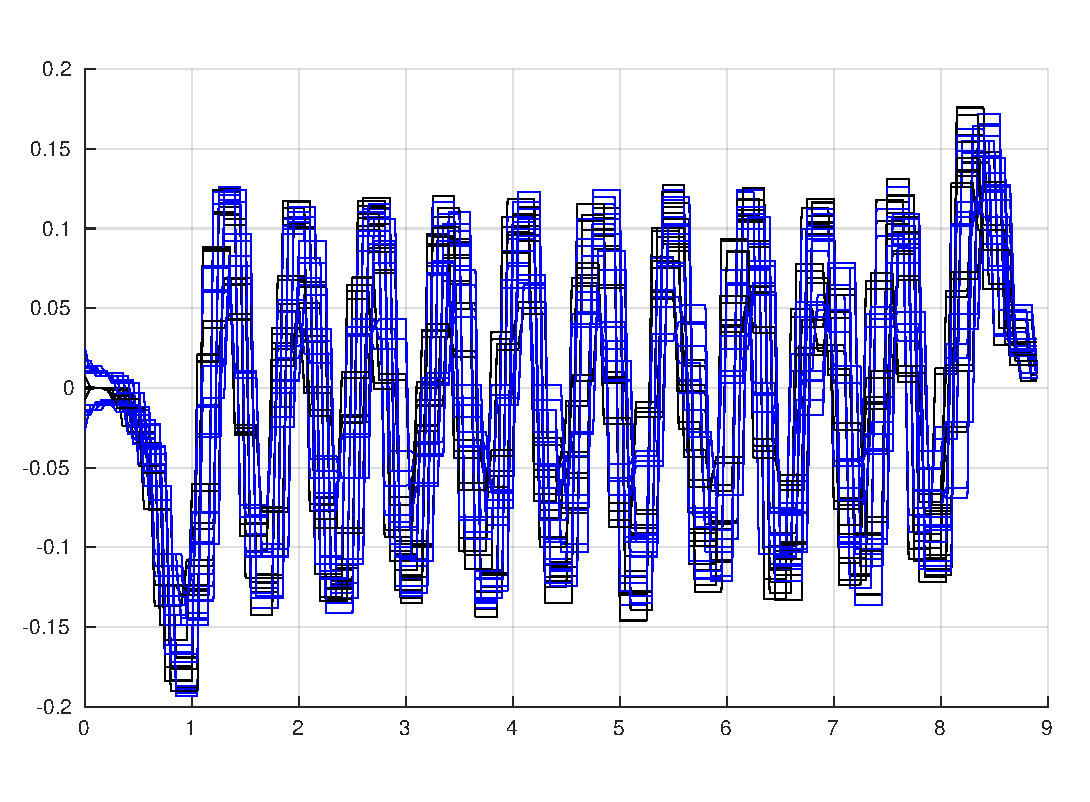
\includegraphics[width=1\linewidth]{Bilder/AnkleRoll_beide_act_sens_links_anfang.pdf}
%	\caption{AnkleRoll Aktoren beider Seiten mit dem Position/Actuator Messwert in schwarz und dem Position/Sensor Messwert in blau. Nao macht hier den ersten Schritt mit Links.}
%	\label{AnkleRoll_beide_act_sens_links_anfang}
%\end{figure}
%\begin{figure}[tb]
%	\centering
%	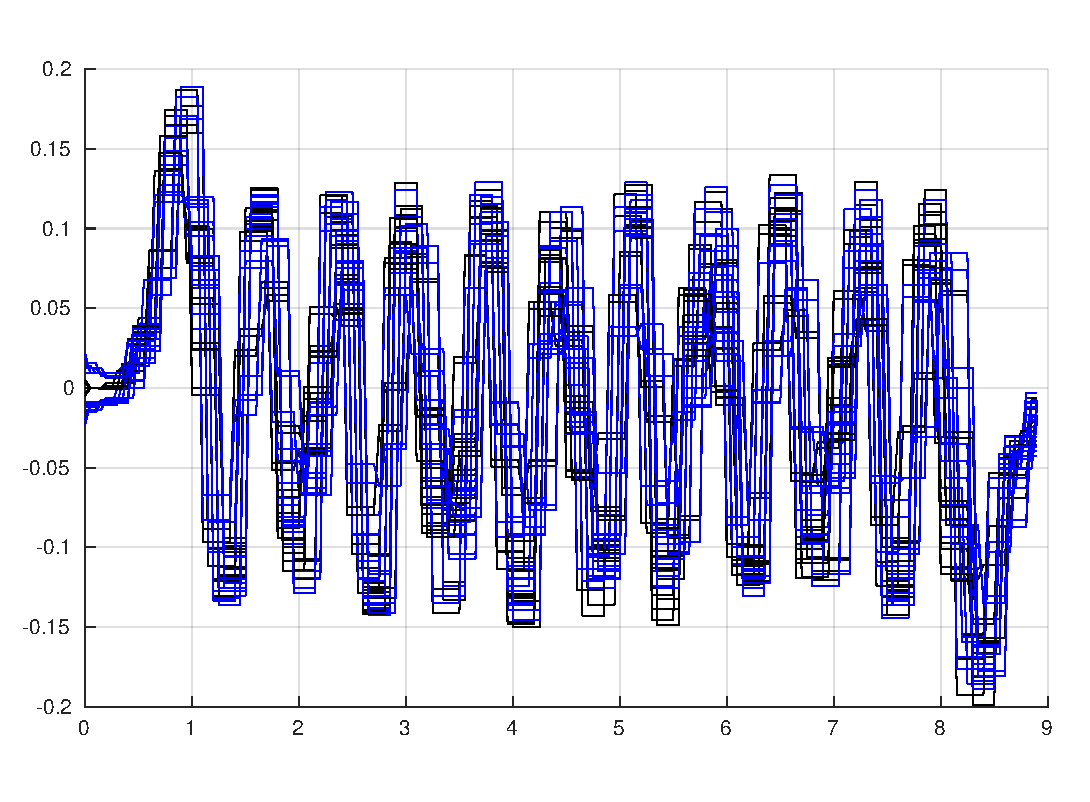
\includegraphics[width=1\linewidth]{Bilder/AnkleRoll_beide_act_sens_rechts_anfang.pdf}
%	\caption{AnkleRoll Aktoren beider Seiten mit dem Position/Actuator Messwert in schwarz und dem Position/Sensor Messwert in blau. Nao macht hier den ersten Schritt mit Rechts.}
%	\label{AnkleRoll_beide_act_sens_rechts_anfang}
%\end{figure}
%\begin{figure}[tb]
%	\centering
%	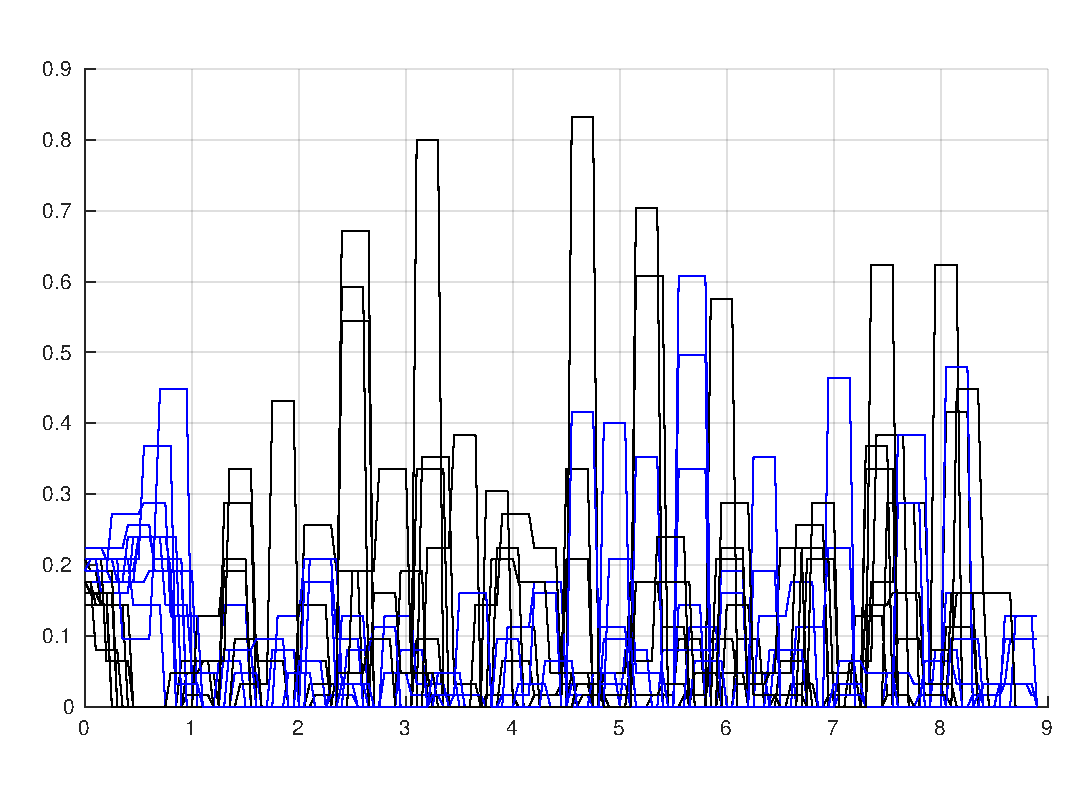
\includegraphics[width=1\linewidth]{Bilder/AnkleRoll_beide_current_links_anfang.pdf}
%	\caption{AnkleRoll Aktoren beider Seiten mit dem Current Messwert. Messwert Links ist in Schwarz, Messwert Rechts ist in Blau. Nao macht hier den ersten Schritt mit Links.}
%	\label{AnkleRoll_beide_current_links_anfang}
%\end{figure}
%\begin{figure}[tb]
%	\centering
%	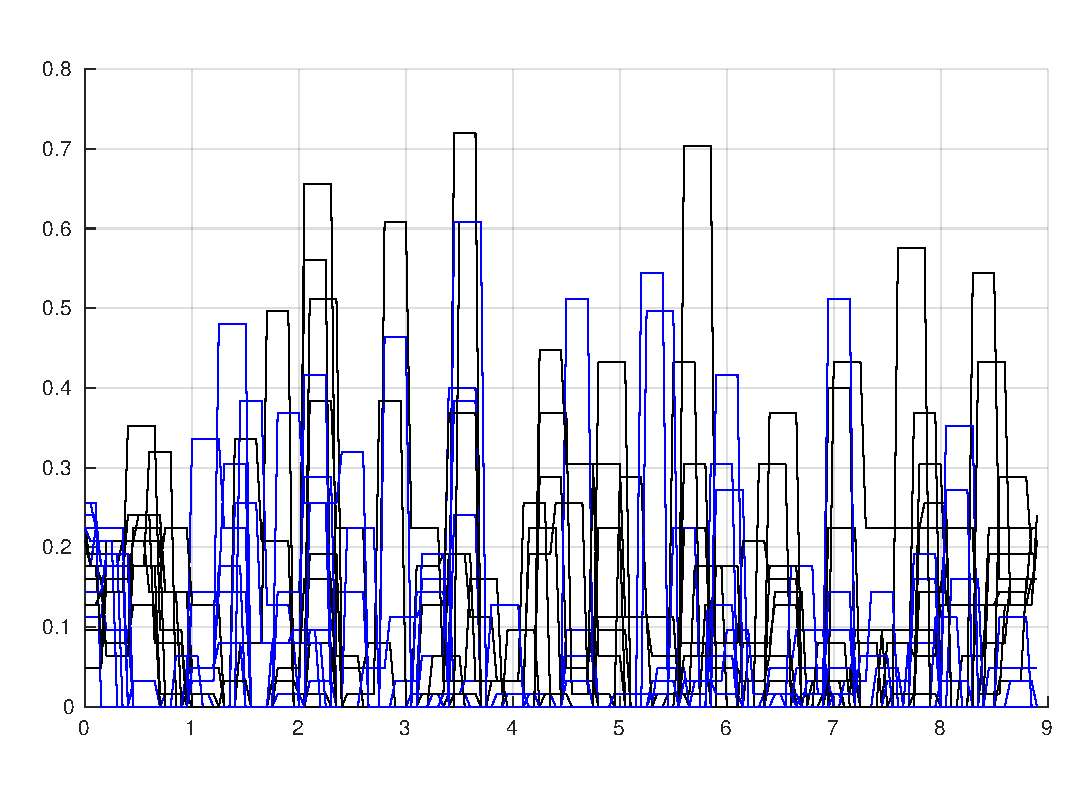
\includegraphics[width=1\linewidth]{Bilder/AnkleRoll_beide_current_rechts_anfang.pdf}
%	\caption{AnkleRoll Aktoren beider Seiten mit dem Current Messwert. Messwert Links ist in Schwarz, Messwert Rechts ist in Blau. Nao macht hier den ersten Schritt mit Rechts.}
%	\label{AnkleRoll_beide_current_rechts_anfang}
%\end{figure}

%%% Local Variables:
%%% mode: latex
%%% TeX-master: "main"
%%% End: